\documentclass[a4paper]{article}
\usepackage{tikz, rotating}
\usetikzlibrary{fadings}
\begin{document}
	\thispagestyle{empty}
	\begin{sidewaysfigure}
		\begin{tikzpicture}[remember picture, overlay] 
			\node[
				inner sep=0pt, 
				opacity=0.5, 
				fill=teal!40 % muda a cor da imagem
			] at (10.6, 0) {
				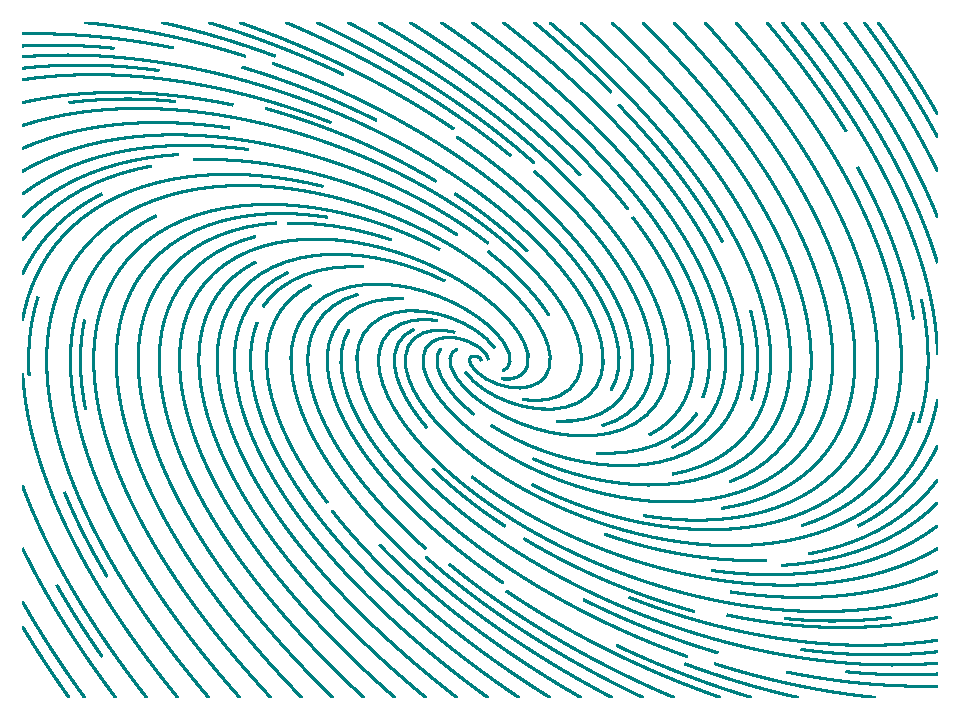
\includegraphics[%
					height=0.78\paperheight,%
				    keepaspectratio
				]{retrato da capa.pdf}
			};
		\begin{scope}[rotate=-90]
			% faixa principal
			\fill [teal!50, opacity=0.9]
				(-11, 8.5) rectangle ++(22, 5)
			;
			\fill [teal!50!black, opacity=0.35]
				(-11, 10.25) rectangle ++(22, 1.5)
			;
			\draw (0, 12.5) node {%
				\Huge\rotatebox{-90}{%
					Técnicas não lineares em Controle
				}
			};
			\draw (0, 11) node {%
				\Huge\rotatebox{-90}{%
					Exercícios
				}
			};
			\draw (0, 9.5) node {%
				\Large\rotatebox{-90}{%
					Prof. Dr. Eugênio L. F. Feitosa
				}
			};
			
			% autor
			\fill [teal!50, opacity=0.95, path fading=north]
				(11, 0) rectangle ++(-40, 1.5)
			;
			\draw (5.5, 1) node [anchor=east] {%
				\large\rotatebox{-90}{%
					Sugestões de soluções por Thiago Tomás de Paula
				}
			};
		\end{scope}
		\end{tikzpicture}
	\end{sidewaysfigure}
\end{document}